\chapter{Конструкторская часть}
В этом разделе будут приведены требования к вводу и программе, а также схемы алгоритмов нахождения расстояний Левенштейна и Дамерау-Левенштейна.

\section{Требования к вводу}
Выделены следующие требования.
\begin{enumerate}
	\item На вход подаются две строки.
	\item Буквы верхнего и нижнего регистров считаются различными.
\end{enumerate}

\section{Требования к программе}
Выделены следующие требования.
\begin{enumerate}
	\item Две пустые строки --- корректный ввод, программа не должна аварийно завершаться.
	\item На выход программа должна вывести число --- расстояние Левенштейна (Дамерау-Левенштейна), матрицу, если она используется алгоритмом.
\end{enumerate}

\section{Разработка алгоритма нахождения расстояния Левенштейна}

На рисунке \ref{fig:levmat} приведена схема алгоритма нахождения расстояния Левенштейна с заполнением матрицы.
\begin{figure}[H]
	\centering
	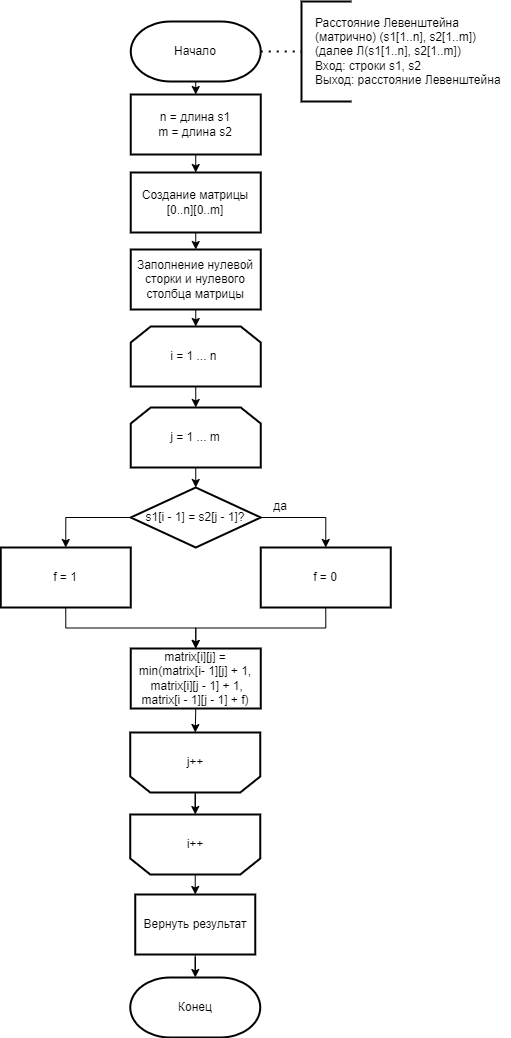
\includegraphics[width=0.7\linewidth]{inc/img/lev_mat}
	\caption{Схема матричного алгоритма нахождения расстояния Левенштейна}
	\label{fig:levmat}
\end{figure}

\section{Разработка алгоритмов нахождения расстояния Дамерау-Левенштейна}
На рисунке \ref{fig:damlevmat} приведена схема алгоритма нахождения расстояния Да- мерау-Левенштейна с заполнением матрицы.
На рисунке \ref{fig:recdamlev} приведена схема алгоритма нахождения расстояния Дамерау-Левенштейна рекурсивно.
\begin{figure}[H]
	\centering
	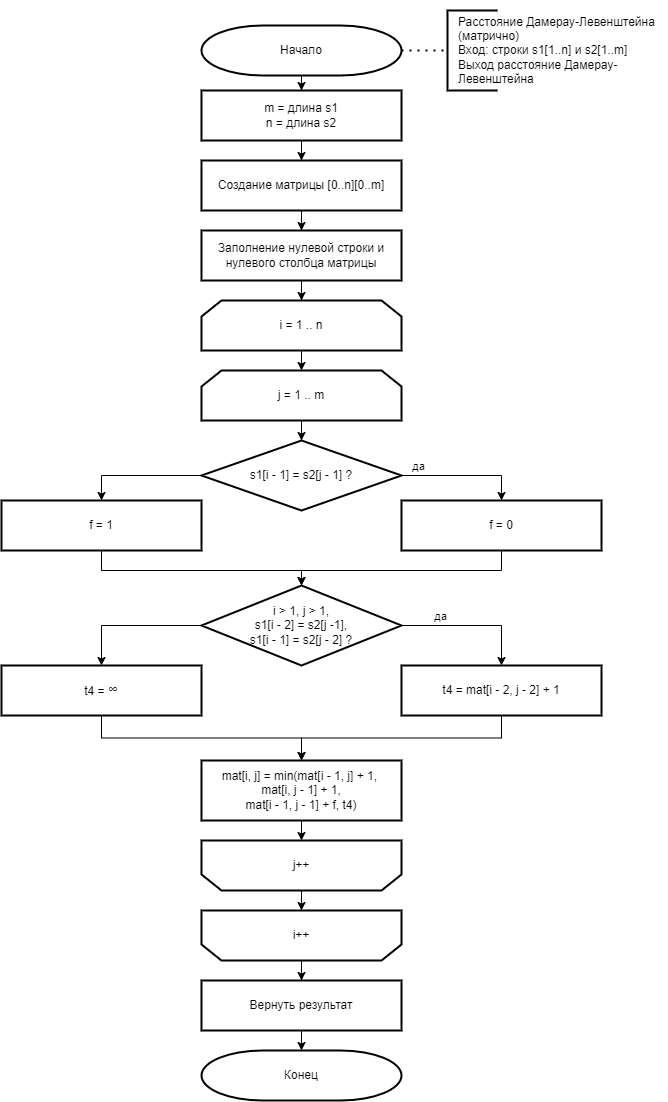
\includegraphics[width=0.7\linewidth]{inc/img/dam_lev_mat}
	\caption{Схема матричного алгоритма нахождения расстояния Дамерау-Левенштейна}
	\label{fig:damlevmat}
\end{figure}
\begin{figure}[H]
	\centering
	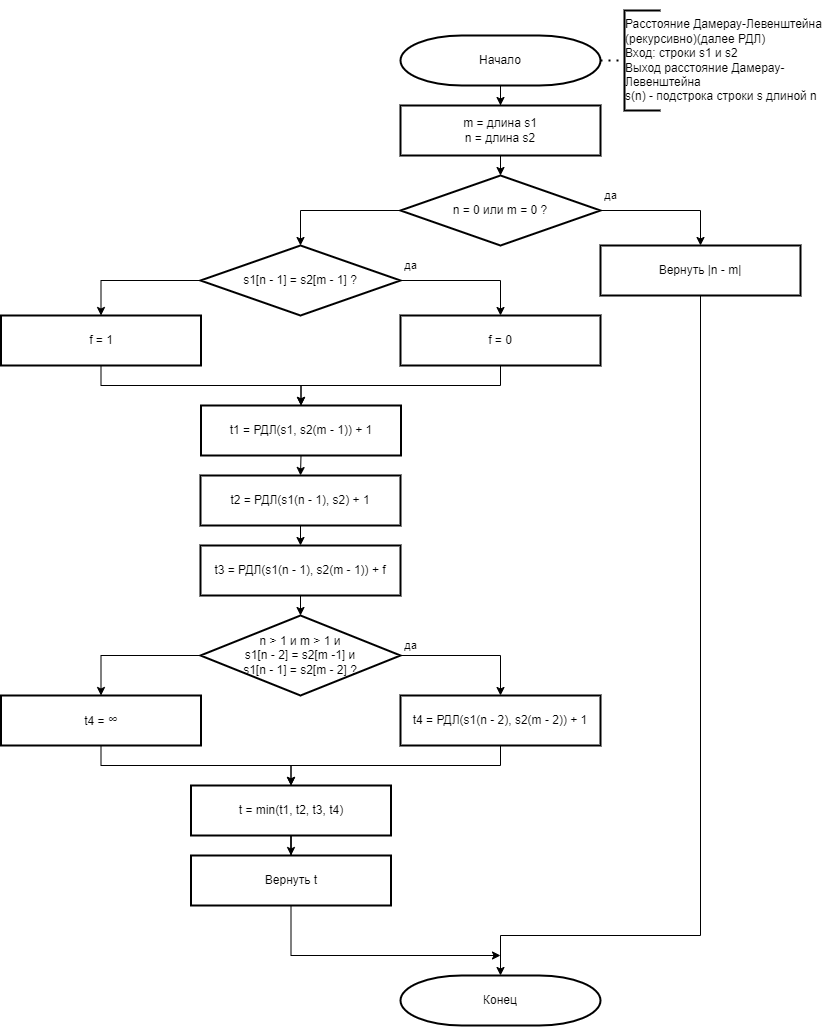
\includegraphics[width=0.7\linewidth]{inc/img/recdamlev}
	\caption{Схема рекурсивного алгоритма нахождения расстояния Дамерау-Левенштейна}
	\label{fig:recdamlev}
\end{figure}

\section*{Вывод}

Перечислены требования к вводу и программе, а также на основе теоретических данных, полученных из аналитического раздела были построены схемы требуемых алгоритмов.





